\documentclass[12pt,a4paper]{report}
\usepackage[utf8]{inputenc}
\usepackage[T1]{fontenc}
\usepackage{lmodern}
\usepackage[margin=1in]{geometry}
\usepackage{graphicx}
\usepackage{hyperref}
\usepackage{listings}
\usepackage{xcolor}
\usepackage{tikz}
\usepackage{booktabs}
\usepackage{longtable}
\usepackage{enumitem}
\usepackage{fancyhdr}
\usepackage{float}

\usetikzlibrary{shapes.geometric, arrows.meta, positioning, fit}

\definecolor{codegreen}{rgb}{0,0.6,0}
\definecolor{codegray}{rgb}{0.5,0.5,0.5}
\definecolor{codepurple}{rgb}{0.58,0,0.82}
\definecolor{backcolour}{rgb}{0.95,0.95,0.95}

\lstdefinestyle{codestyle}{
    backgroundcolor=\color{backcolour},
    commentstyle=\color{codegreen},
    keywordstyle=\color{codepurple}\bfseries,
    numberstyle=\tiny\color{codegray},
    stringstyle=\color{codegreen},
    basicstyle=\ttfamily\small,
    breaklines=true,
    numbers=left,
    numbersep=5pt,
    frame=single,
    tabsize=2
}
\lstset{style=codestyle}

\pagestyle{fancy}
\fancyhf{}
\fancyhead[L]{\leftmark}
\fancyhead[R]{Online Compiler}
\fancyfoot[C]{\thepage}

\hypersetup{colorlinks=true, linkcolor=blue!70!black, urlcolor=blue!70!black}

\tikzstyle{process} = [rectangle, rounded corners, minimum width=2.5cm, minimum height=1cm, text centered, draw=black, fill=blue!15]
\tikzstyle{datastore} = [rectangle, minimum width=2.5cm, minimum height=0.8cm, text centered, draw=black, fill=green!10]
\tikzstyle{entity} = [rectangle, minimum width=2cm, minimum height=1cm, text centered, draw=black, fill=orange!15]
\tikzstyle{component} = [rectangle, rounded corners, minimum width=3cm, minimum height=1cm, text centered, draw=black!70, fill=cyan!10]
\tikzstyle{arrow} = [thick,->,>=stealth]

\begin{document}

%% TITLE PAGE
\begin{titlepage}
\centering
\vspace*{2cm}
{\Huge\bfseries Online Compiler\par}
\vspace{0.5cm}
{\Large\itshape A High-Performance Web-Based Code Execution Platform\par}
\vspace{2cm}
{\large\bfseries Project Documentation \& System Design Report\par}
\vspace{2cm}
\begin{tabular}{ll}
\textbf{Technology:} & C++17, Crow Framework, Docker, SQLite \\
\textbf{Platform:} & Linux / macOS \\
\textbf{Version:} & 1.0 \\
\textbf{Date:} & \today \\
\end{tabular}
\vfill
{\small Comprehensive project report: system design, DFDs, database schema, user manual, deployment.}
\end{titlepage}

\tableofcontents
\newpage

%% ============================================
%% CHAPTER 1: INTRODUCTION
%% ============================================
\chapter{Introduction}

\section{Project Overview}
The \textbf{Online Compiler} is a web-based platform that allows users to write, compile, and execute code in multiple programming languages from their browser. The server is written in \textbf{C++17} for maximum performance, using the Crow web framework for HTTP handling.

Code is executed inside isolated \textbf{Docker containers} with strict resource limits (CPU, memory, PIDs, network), ensuring security. The platform supports \textbf{C++}, \textbf{Python}, and \textbf{JavaScript}.

\section{Problem Statement}
Traditional online compilers use interpreted runtimes (Node.js, Python/Flask) which have:
\begin{itemize}
    \item High memory overhead (50--200MB baseline)
    \item Slow request routing and serialization
    \item Event-loop limitations under concurrent load
\end{itemize}
This project addresses these by using compiled C++, achieving sub-millisecond routing, native multithreading, and under 5MB memory footprint.

\section{Objectives}
\begin{enumerate}
    \item Provide a fast, secure online code execution environment
    \item Support multiple languages (C++, Python, JavaScript)
    \item Isolate execution in Docker sandboxes with resource limits
    \item Implement a modern web UI with syntax highlighting
    \item Store submission history in SQLite database
    \item Package for one-command deployment via Docker Compose
\end{enumerate}

\section{Scope}
\begin{itemize}
    \item \textbf{In Scope:} Code execution, I/O handling, syntax-highlighted editor, submission storage, containerized deployment, rate limiting, timeout enforcement
    \item \textbf{Out of Scope:} User authentication, collaborative editing, real-time sharing, IDE debugging, package installation in containers
\end{itemize}

%% ============================================
%% CHAPTER 2: TECHNOLOGY STACK
%% ============================================
\chapter{Technology Stack}

\section{Backend Technologies}
\begin{longtable}{@{}p{3.5cm}p{3.5cm}p{7cm}@{}}
\toprule
\textbf{Component} & \textbf{Technology} & \textbf{Rationale} \\
\midrule
Language & C++17 & Compiled, zero-overhead, native threading \\
Web Framework & Crow & Header-only, Flask-like API, high throughput \\
Networking & Asio (standalone) & Async I/O, cross-platform, no Boost \\
Build System & CMake 3.14+ & FetchContent for dependency management \\
Process Control & POSIX syscalls & fork, execvp, waitpid, select, pipe \\
Database & SQLite 3 & Embedded, zero-config, ACID compliant \\
\bottomrule
\end{longtable}

\section{Frontend Technologies}
\begin{longtable}{@{}p{3.5cm}p{3.5cm}p{7cm}@{}}
\toprule
\textbf{Component} & \textbf{Technology} & \textbf{Rationale} \\
\midrule
Code Editor & CodeMirror 5 & Syntax highlighting, 100+ modes, lightweight \\
Theme & Dracula & Dark theme, high contrast \\
Styling & Custom CSS & Dark UI, responsive, side-by-side panels \\
API Calls & Fetch API & Native browser API, no dependencies \\
\bottomrule
\end{longtable}

\section{Infrastructure}
\begin{longtable}{@{}p{3.5cm}p{3.5cm}p{7cm}@{}}
\toprule
\textbf{Component} & \textbf{Technology} & \textbf{Rationale} \\
\midrule
Sandboxing & Docker & Process isolation, resource limits \\
Images & gcc, python:3-slim, node:20-slim & Official, minimal \\
Deployment & Docker Compose & One-command multi-container startup \\
\bottomrule
\end{longtable}

%% ============================================
%% CHAPTER 3: SYSTEM ARCHITECTURE
%% ============================================
\chapter{System Architecture}

\section{High-Level Architecture Diagram}

\begin{figure}[H]
\centering
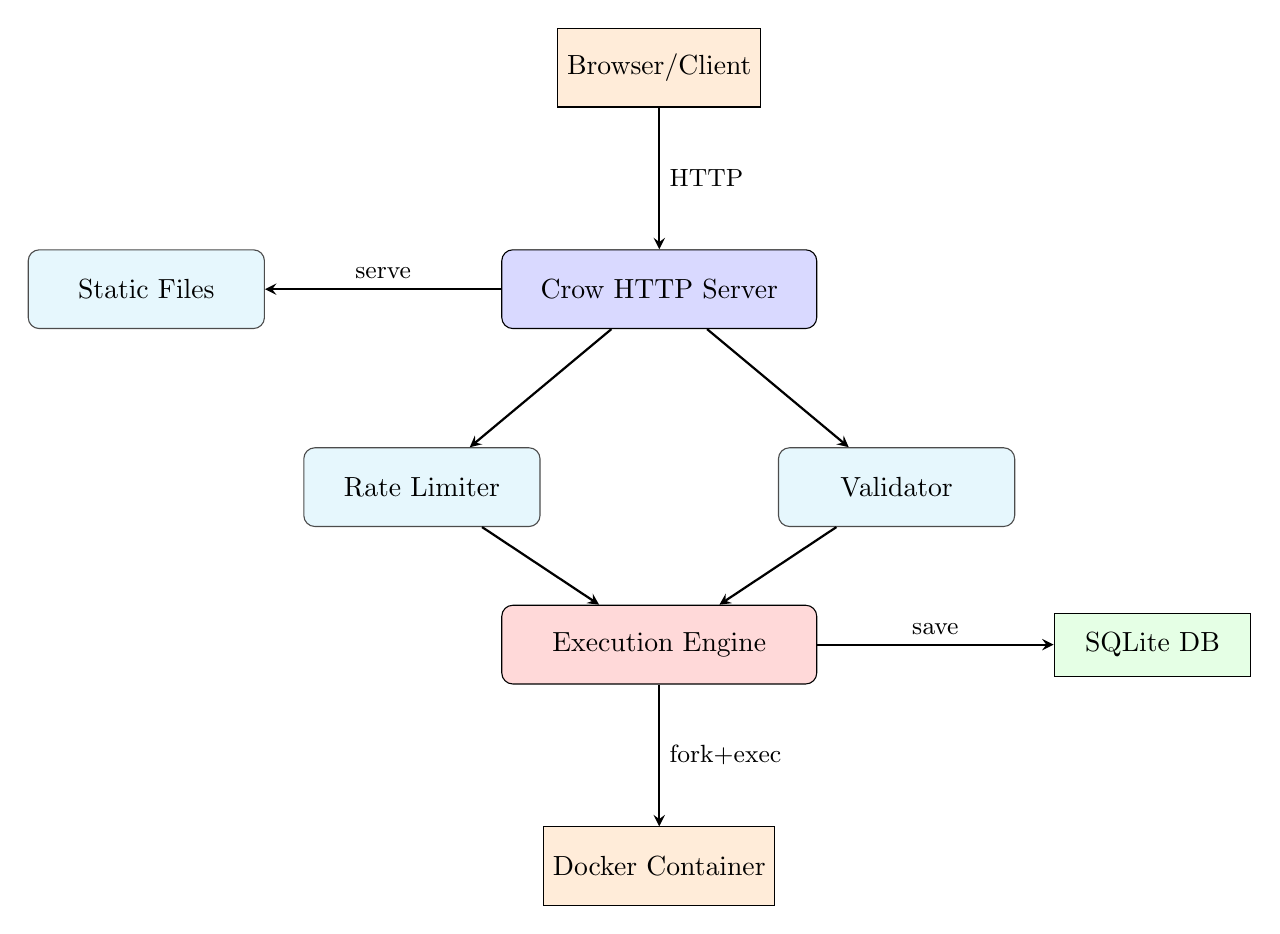
\begin{tikzpicture}[node distance=1.8cm]
    \node (user) [entity] {Browser/Client};
    \node (crow) [process, below=of user, minimum width=4cm] {Crow HTTP Server};
    \node (rate) [component, below left=1.5cm and -0.5cm of crow] {Rate Limiter};
    \node (valid) [component, below right=1.5cm and -0.5cm of crow] {Validator};
    \node (exec) [process, below=3.5cm of crow, minimum width=4cm, fill=red!15] {Execution Engine};
    \node (docker) [entity, below=of exec] {Docker Container};
    \node (db) [datastore, right=3cm of exec] {SQLite DB};
    \node (static) [component, left=3cm of crow] {Static Files};

    \draw [arrow] (user) -- node[right, font=\small] {HTTP} (crow);
    \draw [arrow] (crow) -- (rate);
    \draw [arrow] (crow) -- (valid);
    \draw [arrow] (rate) -- (exec);
    \draw [arrow] (valid) -- (exec);
    \draw [arrow] (exec) -- node[right, font=\small] {fork+exec} (docker);
    \draw [arrow] (exec) -- node[above, font=\small] {save} (db);
    \draw [arrow] (crow) -- node[above, font=\small] {serve} (static);
\end{tikzpicture}
\caption{High-Level System Architecture}
\end{figure}

\section{Component Descriptions}

\subsection{Crow HTTP Server (main.cpp)}
\begin{itemize}
    \item Listens on configurable port (default 3000)
    \item Serves static frontend files
    \item Routes API requests to handlers
    \item Multithreaded (10 threads by default)
    \item Graceful shutdown on SIGINT/SIGTERM
\end{itemize}

\subsection{Execution Engine (executor.cpp)}
For each request:
\begin{enumerate}
    \item Creates unique temporary directory (random hex session ID)
    \item Writes source code and input to files
    \item Constructs \texttt{docker run} command with security flags
    \item Forks child process, uses \texttt{execvp} to launch Docker
    \item Reads stdout/stderr via pipes using \texttt{select()} (deadlock-free)
    \item Enforces timeout via deadline with \texttt{SIGKILL}
    \item Cleans up temporary directory
\end{enumerate}

\subsection{Rate Limiter (rate\_limiter.cpp)}
\begin{itemize}
    \item Thread-safe per-IP fixed-window algorithm
    \item Uses \texttt{std::mutex} for Crow's thread pool
    \item Auto-purges stale entries every 100 requests
\end{itemize}

\subsection{Validator (validator.hpp)}
\begin{itemize}
    \item Checks required fields: language, code
    \item Validates types (must be strings)
    \item Verifies language is supported
    \item Rejects empty code
\end{itemize}

\section{Security Architecture}

\begin{figure}[H]
\centering
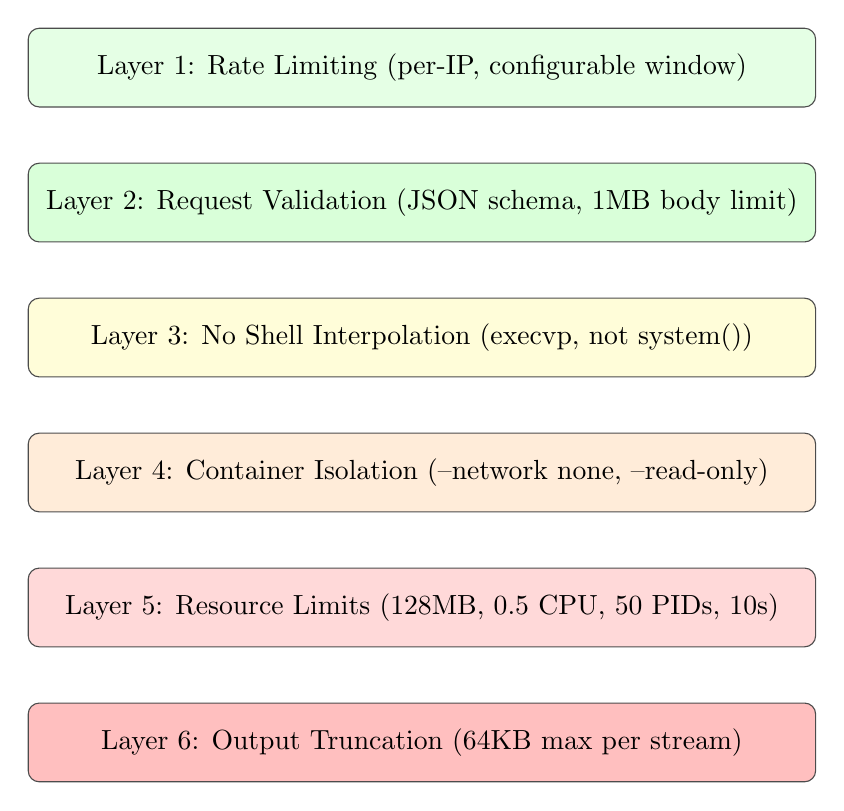
\begin{tikzpicture}[node distance=0.7cm]
    \node (l1) [component, minimum width=10cm, fill=green!10] {Layer 1: Rate Limiting (per-IP, configurable window)};
    \node (l2) [component, minimum width=10cm, fill=green!15, below=of l1] {Layer 2: Request Validation (JSON schema, 1MB body limit)};
    \node (l3) [component, minimum width=10cm, fill=yellow!15, below=of l2] {Layer 3: No Shell Interpolation (execvp, not system())};
    \node (l4) [component, minimum width=10cm, fill=orange!15, below=of l3] {Layer 4: Container Isolation (--network none, --read-only)};
    \node (l5) [component, minimum width=10cm, fill=red!15, below=of l4] {Layer 5: Resource Limits (128MB, 0.5 CPU, 50 PIDs, 10s)};
    \node (l6) [component, minimum width=10cm, fill=red!25, below=of l5] {Layer 6: Output Truncation (64KB max per stream)};
\end{tikzpicture}
\caption{Defense-in-Depth Security Layers}
\end{figure}

Docker security flags per container:
\begin{lstlisting}[language=bash]
docker run --rm --network none --memory 128m --cpus 0.5 \
  --pids-limit 50 --read-only --tmpfs /tmp:size=16m \
  -v <session>:/workspace -w /workspace <image> /bin/sh -c "<cmd>"
\end{lstlisting}

%% ============================================
%% CHAPTER 4: DATA FLOW DIAGRAMS
%% ============================================
\chapter{Data Flow Diagrams}

\section{Level 0 DFD (Context Diagram)}

\begin{figure}[H]
\centering
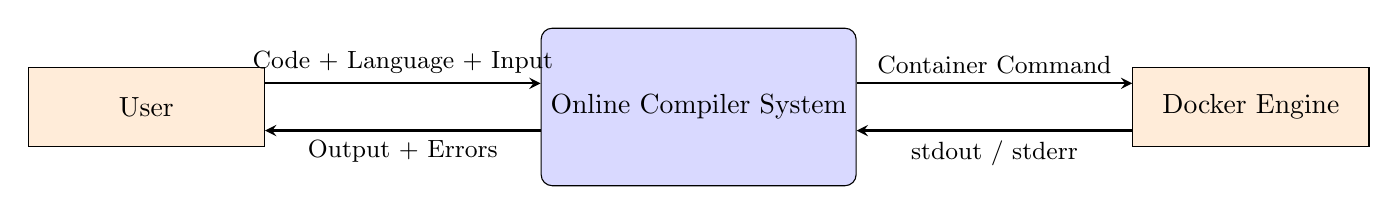
\begin{tikzpicture}[node distance=3.5cm]
    \node (user) [entity, minimum width=3cm] {User};
    \node (system) [process, right=of user, minimum width=4cm, minimum height=2cm] {Online Compiler System};
    \node (docker) [entity, right=of system, minimum width=3cm] {Docker Engine};

    \draw [arrow] ([yshift=3mm]user.east) -- node[above, font=\small] {Code + Language + Input} ([yshift=3mm]system.west);
    \draw [arrow] ([yshift=-3mm]system.west) -- node[below, font=\small] {Output + Errors} ([yshift=-3mm]user.east);
    \draw [arrow] ([yshift=3mm]system.east) -- node[above, font=\small] {Container Command} ([yshift=3mm]docker.west);
    \draw [arrow] ([yshift=-3mm]docker.west) -- node[below, font=\small] {stdout / stderr} ([yshift=-3mm]system.east);
\end{tikzpicture}
\caption{Level 0 DFD --- Context Diagram}
\end{figure}

\section{Level 1 DFD}

\begin{figure}[H]
\centering
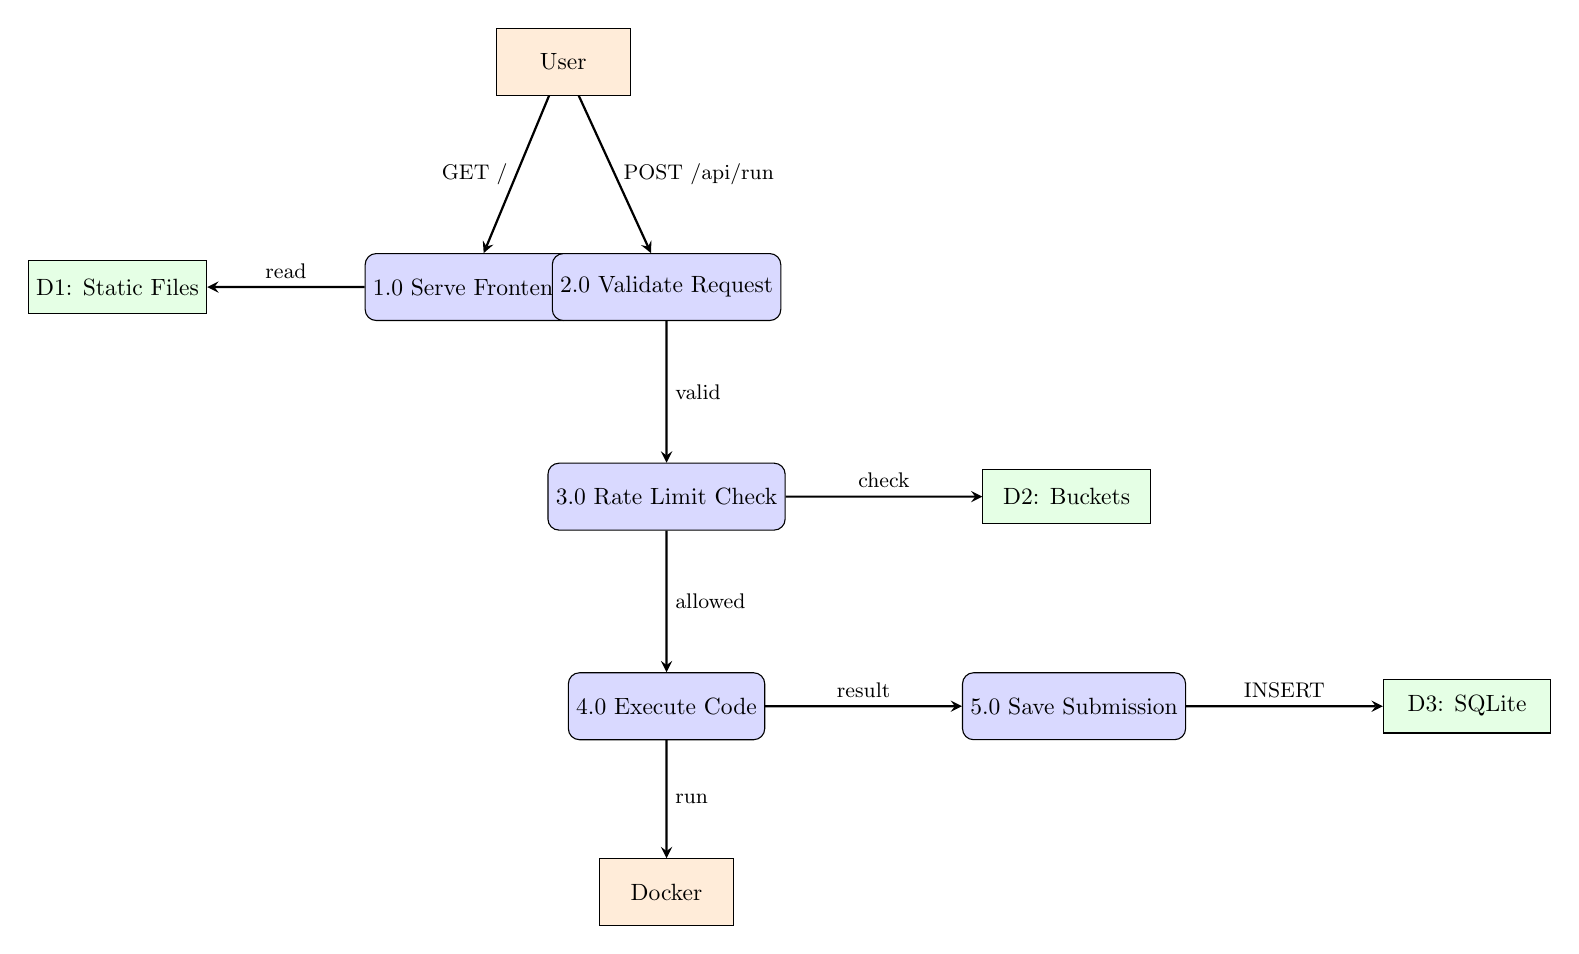
\begin{tikzpicture}[node distance=1.5cm, scale=0.85, every node/.style={scale=0.85}]
    \node (user) [entity] {User};
    \node (p1) [process, below left=2cm and -1cm of user] {1.0 Serve Frontend};
    \node (p2) [process, below right=2cm and -1cm of user] {2.0 Validate Request};
    \node (p3) [process, below=1.8cm of p2] {3.0 Rate Limit Check};
    \node (p4) [process, below=1.8cm of p3] {4.0 Execute Code};
    \node (p5) [process, right=2.5cm of p4] {5.0 Save Submission};

    \node (d1) [datastore, left=2cm of p1] {D1: Static Files};
    \node (d2) [datastore, right=2.5cm of p3] {D2: Buckets};
    \node (d3) [datastore, right=2.5cm of p5] {D3: SQLite};
    \node (docker) [entity, below=1.5cm of p4] {Docker};

    \draw [arrow] (user) -- node[left, font=\small] {GET /} (p1);
    \draw [arrow] (p1) -- node[above, font=\small] {read} (d1);
    \draw [arrow] (user) -- node[right, font=\small] {POST /api/run} (p2);
    \draw [arrow] (p2) -- node[right, font=\small] {valid} (p3);
    \draw [arrow] (p3) -- node[above, font=\small] {check} (d2);
    \draw [arrow] (p3) -- node[right, font=\small] {allowed} (p4);
    \draw [arrow] (p4) -- node[right, font=\small] {run} (docker);
    \draw [arrow] (p4) -- node[above, font=\small] {result} (p5);
    \draw [arrow] (p5) -- node[above, font=\small] {INSERT} (d3);
\end{tikzpicture}
\caption{Level 1 DFD --- Major Processes}
\end{figure}

\section{Level 2 DFD --- Execution Engine}

\begin{figure}[H]
\centering
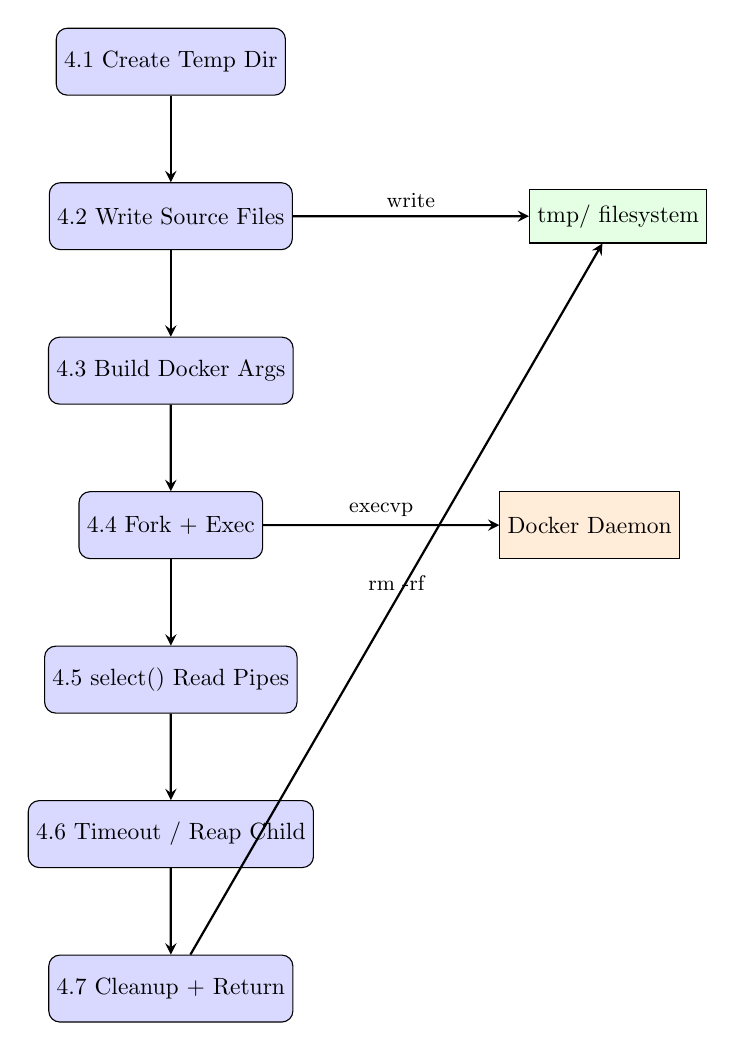
\begin{tikzpicture}[node distance=1.1cm, scale=0.85, every node/.style={scale=0.85}]
    \node (p1) [process] {4.1 Create Temp Dir};
    \node (p2) [process, below=of p1] {4.2 Write Source Files};
    \node (p3) [process, below=of p2] {4.3 Build Docker Args};
    \node (p4) [process, below=of p3] {4.4 Fork + Exec};
    \node (p5) [process, below=of p4] {4.5 select() Read Pipes};
    \node (p6) [process, below=of p5] {4.6 Timeout / Reap Child};
    \node (p7) [process, below=of p6] {4.7 Cleanup + Return};

    \node (fs) [datastore, right=3cm of p2] {tmp/ filesystem};
    \node (docker) [entity, right=3cm of p4] {Docker Daemon};

    \draw [arrow] (p1) -- (p2);
    \draw [arrow] (p2) -- (p3);
    \draw [arrow] (p3) -- (p4);
    \draw [arrow] (p4) -- (p5);
    \draw [arrow] (p5) -- (p6);
    \draw [arrow] (p6) -- (p7);
    \draw [arrow] (p2) -- node[above, font=\small] {write} (fs);
    \draw [arrow] (p4) -- node[above, font=\small] {execvp} (docker);
    \draw [arrow] (p7) -- node[above, font=\small] {rm -rf} (fs);
\end{tikzpicture}
\caption{Level 2 DFD --- Execution Engine Detail}
\end{figure}

%% ============================================
%% CHAPTER 5: DATABASE SCHEMA
%% ============================================
\chapter{Database Schema}

\section{Overview}
The system uses \textbf{SQLite 3} as an embedded database for submission history. Chosen for:
\begin{itemize}
    \item Zero configuration --- no separate server
    \item Single-file storage --- easy backup
    \item ACID compliant with WAL mode
    \item Native C API, minimal overhead
\end{itemize}

\section{Table: submissions}

\begin{longtable}{@{}p{2.5cm}p{2.5cm}p{3cm}p{5.5cm}@{}}
\toprule
\textbf{Column} & \textbf{Type} & \textbf{Constraint} & \textbf{Description} \\
\midrule
id & INTEGER & PK AUTOINCREMENT & Unique submission ID \\
language & TEXT & NOT NULL & Language key (cpp/python/javascript) \\
code & TEXT & NOT NULL & Source code submitted \\
input & TEXT & DEFAULT '' & Stdin input \\
stdout & TEXT & DEFAULT '' & Captured standard output \\
stderr & TEXT & DEFAULT '' & Captured standard error \\
exit\_code & INTEGER & DEFAULT 0 & Process exit code \\
timed\_out & INTEGER & DEFAULT 0 & Timeout flag (0/1) \\
created\_at & TEXT & DEFAULT CURRENT\_TIMESTAMP & ISO 8601 timestamp \\
\bottomrule
\end{longtable}

\section{SQL DDL}
\begin{lstlisting}[language=SQL]
CREATE TABLE IF NOT EXISTS submissions (
    id          INTEGER PRIMARY KEY AUTOINCREMENT,
    language    TEXT    NOT NULL,
    code        TEXT    NOT NULL,
    input       TEXT    DEFAULT '',
    stdout      TEXT    DEFAULT '',
    stderr      TEXT    DEFAULT '',
    exit_code   INTEGER DEFAULT 0,
    timed_out   INTEGER DEFAULT 0,
    created_at  TEXT    DEFAULT CURRENT_TIMESTAMP
);
CREATE INDEX IF NOT EXISTS idx_lang ON submissions(language);
CREATE INDEX IF NOT EXISTS idx_time ON submissions(created_at);
\end{lstlisting}

%% ============================================
%% CHAPTER 6: API DOCUMENTATION
%% ============================================
\chapter{API Documentation}

\section{Base URL}
\texttt{http://localhost:3000}

\section{Endpoints}

\subsection{GET /}
Returns the frontend HTML page.

\subsection{GET /public/<path>}
Serves static assets (CSS, JS). Path traversal is blocked.

\subsection{POST /api/run}
Execute code in a sandboxed container.

\textbf{Request Headers:}
\begin{lstlisting}
Content-Type: application/json
\end{lstlisting}

\textbf{Request Body:}
\begin{lstlisting}[language=json]
{
  "language": "python",
  "code": "print('hello')",
  "input": "optional stdin"
}
\end{lstlisting}

\textbf{Success Response (200):}
\begin{lstlisting}[language=json]
{
  "stdout": "hello\n",
  "stderr": "",
  "exitCode": 0,
  "timedOut": false
}
\end{lstlisting}

\textbf{Error Responses:}
\begin{itemize}
    \item \textbf{400} --- Invalid request (missing fields, unsupported language, empty code)
    \item \textbf{413} --- Request body exceeds 1MB
    \item \textbf{429} --- Rate limit exceeded
\end{itemize}

\subsection{GET /api/submissions}
Retrieve recent submissions.

\textbf{Query Parameters:}
\begin{itemize}
    \item \texttt{limit} --- Max results (default 20, max 100)
    \item \texttt{language} --- Filter by language (optional)
\end{itemize}

\textbf{Response (200):}
\begin{lstlisting}[language=json]
{
  "submissions": [
    {
      "id": 1,
      "language": "python",
      "code": "print('hi')",
      "stdout": "hi\n",
      "exitCode": 0,
      "createdAt": "2025-01-15 10:30:00"
    }
  ]
}
\end{lstlisting}

%% ============================================
%% CHAPTER 7: USER MANUAL
%% ============================================
\chapter{User Manual}

\section{Getting Started}
\begin{enumerate}
    \item Open \texttt{http://localhost:3000} in a modern browser (Chrome, Firefox, Safari, Edge).
    \item The editor loads with a default ``Hello World'' C++ program.
\end{enumerate}

\section{Writing Code}
\begin{enumerate}
    \item Select a language from the dropdown (C++, Python, JavaScript).
    \item The editor automatically switches syntax highlighting mode and loads a starter template.
    \item Type or paste your code in the editor panel (left side).
    \item Features: line numbers, bracket matching, auto-indent, Tab inserts 4 spaces.
\end{enumerate}

\section{Providing Input}
If your program reads from stdin, type the input in the ``Stdin Input'' textarea below the editor.

\section{Running Code}
\begin{itemize}
    \item Click the \textbf{Run} button, OR
    \item Press \textbf{Ctrl+Enter} (Windows/Linux) or \textbf{Cmd+Enter} (macOS).
\end{itemize}

\section{Viewing Results}
\begin{itemize}
    \item \textbf{Output panel} (right side, green text): Shows stdout from your program.
    \item \textbf{Errors panel} (right side, red text): Shows stderr (compilation errors, runtime errors).
    \item \textbf{Status indicator}: Shows execution time or error status.
\end{itemize}

\section{Clearing}
Click \textbf{Clear} to reset the editor to the default template and clear all output.

\section{Limitations}
\begin{itemize}
    \item Maximum execution time: 10 seconds
    \item Maximum output: 64KB per stream
    \item Maximum code size: 1MB
    \item Rate limit: 10 requests per 60 seconds
    \item No file I/O beyond stdin/stdout
    \item No network access from code
    \item No graphical output
\end{itemize}

%% ============================================
%% CHAPTER 8: DEPLOYMENT GUIDE
%% ============================================
\chapter{Deployment Guide}

\section{Prerequisites}
\begin{itemize}
    \item Docker Engine 20+ installed and running
    \item Docker Compose v2+ (or docker-compose v1.29+)
    \item At least 512MB RAM available
    \item Ports 3000 available (configurable)
\end{itemize}

\section{Quick Start with Docker Compose}
\begin{lstlisting}[language=bash]
git clone <repository-url>
cd OnlineCompiler
docker compose up --build
\end{lstlisting}
This builds the server image and starts the application. Open \texttt{http://localhost:3000}.

\section{Manual Build (Development)}
\begin{lstlisting}[language=bash]
# Requirements: C++17 compiler, CMake 3.14+, Docker
mkdir build && cd build
cmake ..
make -j$(nproc)          # Linux
make -j$(sysctl -n hw.ncpu)  # macOS
./online_compiler        # Run from build/ directory
\end{lstlisting}

\section{Configuration}
Environment variables (all optional, have defaults):

\begin{longtable}{@{}p{4.5cm}p{2cm}p{7cm}@{}}
\toprule
\textbf{Variable} & \textbf{Default} & \textbf{Description} \\
\midrule
PORT & 3000 & Server listen port \\
DOCKER\_TIMEOUT\_SECONDS & 10 & Max execution time \\
DOCKER\_MEMORY\_LIMIT & 128m & Container memory cap \\
DOCKER\_CPU\_LIMIT & 0.5 & CPU cores per container \\
DOCKER\_PIDS\_LIMIT & 50 & Max processes \\
RATE\_LIMIT\_MAX\_REQUESTS & 10 & Requests per window \\
RATE\_LIMIT\_WINDOW\_SECONDS & 60 & Rate limit window \\
\bottomrule
\end{longtable}

\section{Production Considerations}
\begin{itemize}
    \item Run behind a reverse proxy (nginx/Caddy) for TLS termination
    \item Set resource limits on the server container itself
    \item Monitor disk usage in \texttt{tmp/} directory
    \item Pre-pull Docker images (\texttt{docker pull gcc:latest python:3-slim node:20-slim})
    \item Consider setting \texttt{--log-driver=json-file --log-opts max-size=10m} on containers
\end{itemize}

%% ============================================
%% CHAPTER 9: TESTING
%% ============================================
\chapter{Testing Strategy}

\section{Unit Testing}
\begin{itemize}
    \item \textbf{Validator}: Test all edge cases (empty body, wrong types, unsupported languages)
    \item \textbf{Rate Limiter}: Verify counting, window reset, stale purge
    \item \textbf{Config}: Test env parsing, invalid values fallback
\end{itemize}

\section{Integration Testing}
\begin{lstlisting}[language=bash]
# Valid request
curl -X POST http://localhost:3000/api/run \
  -H 'Content-Type: application/json' \
  -d '{"language":"python","code":"print(42)"}'
# Expected: {"stdout":"42\n","stderr":"","exitCode":0,"timedOut":false}

# Invalid language
curl -X POST http://localhost:3000/api/run \
  -H 'Content-Type: application/json' \
  -d '{"language":"ruby","code":"puts 1"}'
# Expected: 400 {"error":"Unsupported language 'ruby'"}

# Timeout test
curl -X POST http://localhost:3000/api/run \
  -H 'Content-Type: application/json' \
  -d '{"language":"python","code":"import time; time.sleep(20)"}'
# Expected: {"stderr":"Execution timed out","timedOut":true}
\end{lstlisting}

\section{Stress Testing}
\begin{lstlisting}[language=bash]
# Concurrent requests (requires 'hey' or 'ab')
hey -n 50 -c 10 -m POST \
  -H "Content-Type: application/json" \
  -d '{"language":"python","code":"print(1)"}' \
  http://localhost:3000/api/run
\end{lstlisting}

%% ============================================
%% CHAPTER 10: FUTURE ENHANCEMENTS
%% ============================================
\chapter{Future Enhancements}

\begin{enumerate}
    \item \textbf{User Authentication} --- OAuth2/JWT for user accounts and personal submission history
    \item \textbf{More Languages} --- Rust, Go, Java, Ruby, TypeScript
    \item \textbf{Custom Libraries} --- Allow importing common packages (numpy, lodash)
    \item \textbf{Collaboration} --- Real-time shared editing via WebSockets
    \item \textbf{Code Sharing} --- Unique URLs for sharing code snippets
    \item \textbf{Execution Queue} --- Queue-based execution for high load with worker pool
    \item \textbf{Metrics Dashboard} --- Prometheus/Grafana for monitoring
    \item \textbf{File Upload} --- Support multi-file projects
    \item \textbf{CI/CD} --- GitHub Actions for automated testing and deployment
    \item \textbf{Cloud Deployment} --- AWS/GCP with auto-scaling
\end{enumerate}

%% ============================================
%% CHAPTER 11: CONCLUSION
%% ============================================
\chapter{Conclusion}

The Online Compiler project demonstrates that a high-performance, secure code execution platform can be built with minimal dependencies using modern C++. Key achievements:

\begin{itemize}
    \item \textbf{Performance}: Sub-millisecond request routing, 5MB server memory footprint
    \item \textbf{Security}: Six-layer defense-in-depth with Docker isolation
    \item \textbf{Reliability}: Deadlock-free pipe I/O, graceful shutdown, stale resource cleanup
    \item \textbf{Usability}: CodeMirror editor with syntax highlighting, keyboard shortcuts
    \item \textbf{Deployability}: Single Docker Compose command for full-stack deployment
\end{itemize}

The architecture is extensible --- adding new languages requires only a single entry in the language configuration map, and the Docker-based isolation ensures any language runtime is supported without modification to the core engine.

\end{document}
